%%%%%%%%%%%%%%%%%%%%%%%%%%%%%%%%%%%%%%%%%
% Short Sectioned Assignment
% LaTeX Template
% Version 1.0 (5/5/12)
%
% This template has been downloaded from:
% http://www.LaTeXTemplates.com
%
% Original author:
% Frits Wenneker (http://www.howtotex.com)
%
% License:
% CC BY-NC-SA 3.0 (http://creativecommons.org/licenses/by-nc-sa/3.0/)
%
%%%%%%%%%%%%%%%%%%%%%%%%%%%%%%%%%%%%%%%%%

%----------------------------------------------------------------------------------------
%	PACKAGES AND OTHER DOCUMENT CONFIGURATIONS
%----------------------------------------------------------------------------------------

\documentclass[paper=a4, fontsize=11pt]{scrartcl} % A4 paper and 11pt font size

\usepackage[T1]{fontenc} % Use 8-bit encoding that has 256 glyphs
% \usepackage{fourier} % Use the Adobe Utopia font for the document - comment this line to return to the LaTeX default
\usepackage[english]{babel} % English language/hyphenations
\usepackage{amsmath,amsfonts,amsthm} % Math packages

\usepackage{graphicx}
\usepackage{caption}
\usepackage{subcaption}

\usepackage{sectsty} % Allows customizing section commands
\allsectionsfont{\centering \normalfont\scshape} % Make all sections centered, the default font and small caps

\usepackage{fancyhdr} % Custom headers and footers
\pagestyle{fancyplain} % Makes all pages in the document conform to the custom headers and footers
\fancyhead{} % No page header - if you want one, create it in the same way as the footers below
\fancyfoot[L]{} % Empty left footer
\fancyfoot[C]{} % Empty center footer
\fancyfoot[R]{\thepage} % Page numbering for right footer
\renewcommand{\headrulewidth}{0pt} % Remove header underlines
\renewcommand{\footrulewidth}{0pt} % Remove footer underlines
\setlength{\headheight}{13.6pt} % Customize the height of the header

\numberwithin{equation}{section} % Number equations within sections (i.e. 1.1, 1.2, 2.1, 2.2 instead of 1, 2, 3, 4)
\numberwithin{figure}{section} % Number figures within sections (i.e. 1.1, 1.2, 2.1, 2.2 instead of 1, 2, 3, 4)
\numberwithin{table}{section} % Number tables within sections (i.e. 1.1, 1.2, 2.1, 2.2 instead of 1, 2, 3, 4)

\setlength\parindent{0pt} % Removes all indentation from paragraphs - comment this line for an assignment with lots of text

%----------------------------------------------------------------------------------------
%	TITLE SECTION
%----------------------------------------------------------------------------------------

\newcommand{\horrule}[1]{\rule{\linewidth}{#1}} % Create horizontal rule command with 1 argument of height

\title{	
\normalfont \normalsize 
\textsc{Missouri University of Science and Technology} \\ [25pt] % Your university, school and/or department name(s)
\horrule{0.5pt} \\[0.4cm] % Thin top horizontal rule
\huge Structures II: Final Project \\ % The assignment title
\horrule{2pt} \\[0.5cm] % Thick bottom horizontal rule
}

\author{Mitchell Wainwright \\ Ryan Krattiger} % Your name

\date{\normalsize\today} % Today's date or a custom date

\begin{document}

\maketitle % Print the title

%----------------------------------------------------------------------------------------
%	PROBLEM 1
%----------------------------------------------------------------------------------------

\section{Editing Solver Code}

The edited code is available in the github repository found at: \\\\
\textit {https://github.com/rjk9w5/FEM\_project.git} \\


%----------------------------------------------------------------------------------------
%	PROBLEM 2
%----------------------------------------------------------------------------------------
\newpage
\section{Dog-Bone in Uniaxial Tension}

%------------------------------------------------
The Young modulus (E) was calculated for various lengths of L where $L = \beta A$. 'A' is a constant, and $\beta$ was varied as 0.2, 0.5, 1, 2, and 5. The actual Young modulus was 70 GPa. The results are tabulated in table \ref{tab:q2table1} and shown graphically in fig. \ref{fig:q2fig1} and \ref{fig:q2fig2}. \\
\\
It can be seen that the Young modulus is within the desired tolerance when the length is 10x the cross-sectional area. \\
\\
The reason an error occurs in the calculation of the Young modulus is a result of the numerical errors from running the simulation. The longer the dog-bone specimen becomes the closer it matches the assumption of a uniform width rod that is used for calculating the Young modulus in the first place.

\begin{figure}[ht]
	\begin{subfigure}[b]{0.45\textwidth}
		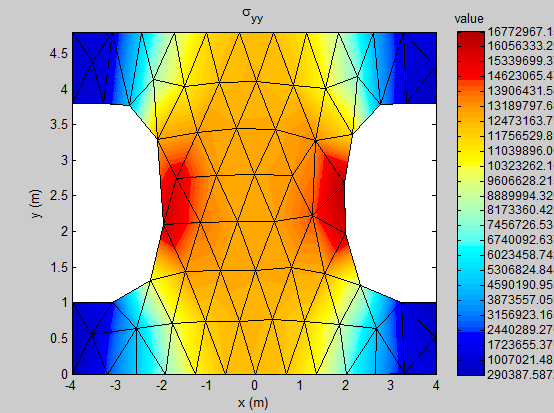
\includegraphics[width=\textwidth]{stress02.png}
		\caption{$L = 0.2 A$}
	\end{subfigure}
	\hfill
	\begin{subfigure}[b]{0.45\textwidth}
		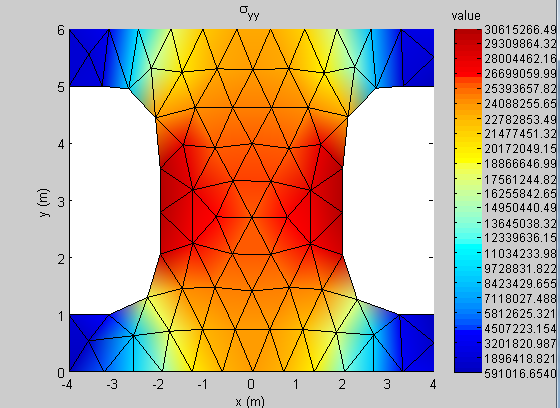
\includegraphics[width=\textwidth]{stress05.png}
		\caption{$L = 0.5 A$}
	\end{subfigure}
	\\
	\begin{subfigure}[b]{0.45\textwidth}
		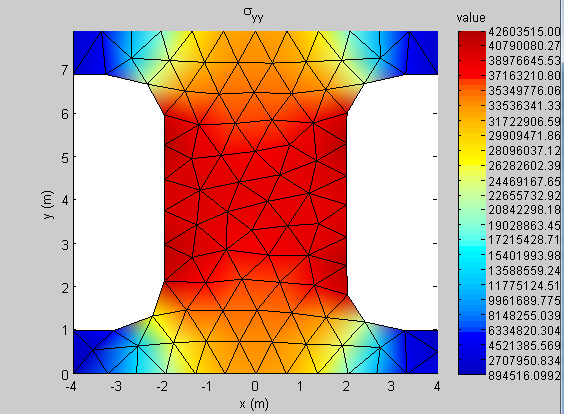
\includegraphics[width=\textwidth]{stress1.png}
		\caption{$L = 1 A$}
	\end{subfigure}
	\hfill
	\begin{subfigure}[b]{0.45\textwidth}
		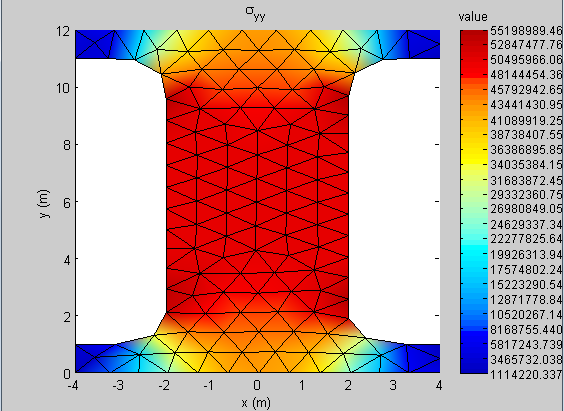
\includegraphics[width=\textwidth]{stress2.png}
		\caption{$L = 2 A$}
	\end{subfigure}
	\\
	\begin{subfigure}[b]{0.45\textwidth}
		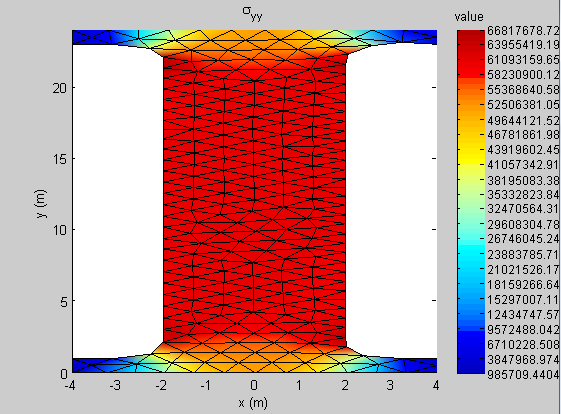
\includegraphics[width=\textwidth]{stress5.png}
		\caption{$L = 5 A$}
	\end{subfigure}
	\hfill
	\begin{subfigure}[b]{0.45\textwidth}
		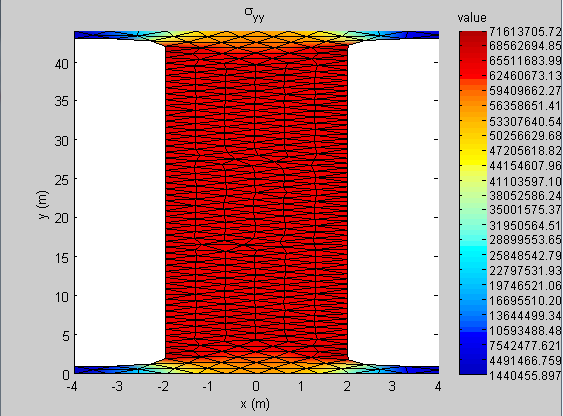
\includegraphics[width=\textwidth]{stress10.png}
		\caption{$L = 10 A$}
	\end{subfigure}
	\caption{Stress Distributions for each Iteration}
\end{figure}

\begin{table}[t]
\centering
	\begin{tabular}{c c c}
		 $\beta$ & E [GPa] & \% error \\
		 \hline
		 0.2 & 14.48 & 79.31 \\
		 0.5 & 27.67 & 60.48\\
		 1 & 39.23 & 43.95\\
		 2 & 50.64 & 27.65\\
		 5 & 60.71 & 13.28\\
		 10 & 65.02 & 7.119\\
		\hline
	\end{tabular}
\caption{Tabulated Results for Calculated Young modulus}
\label{tab:q2table1}
\end{table}

\begin{figure}[h]
\centering
	\begin{subfigure}[b]{0.45\textwidth}
		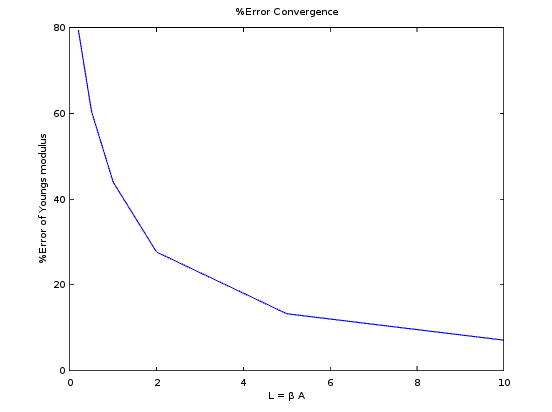
\includegraphics[width=\textwidth]{q2_error.png}
		\caption{Plot of \%error of calculated Young modulus}
		\label{fig:q2fig1}
	\end{subfigure}
	\hfill
	\begin{subfigure}[b]{0.45\textwidth}
		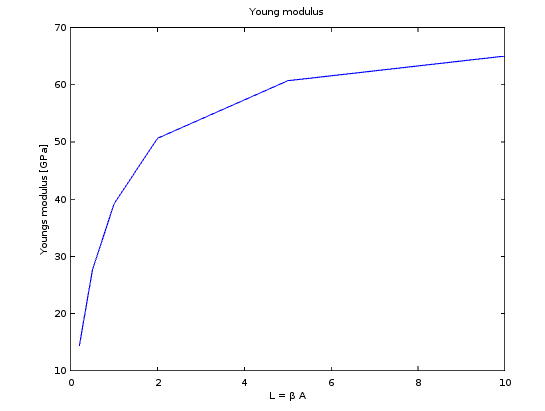
\includegraphics[width=\textwidth]{q2_youngmod.png}
		\caption{Plot of calculated Young modulus}
		\label{fig:q2fig2}
	\end{subfigure}
	\caption{\%Error and value of apparent Young modulus versus gage length}
\end{figure}

%----------------------------------------------------------------------------------------
%	PROBLEM 2
%----------------------------------------------------------------------------------------
\newpage
\section{Flat Plate with a Hole}

%----------------------------------------------------------------------------------------



\end{document}